\documentclass[11pt,a4paper]{article}
\usepackage{amsmath}
\usepackage{array}
\usepackage{graphicx}
\usepackage[utf8]{inputenc}
\usepackage{verbatim}
\usepackage[francais]{babel}
\usepackage{graphicx}

\def\alp{\ensuremath{\alpha} }
%\def\pi{\ensuremath{\pi} }

%\usepackage{minted}
\begin{document}
\title{Rapport de TP SoC/Cache}
\author{Binôme: Bonnardel Julien et Ikhalo Ojeme}
\maketitle
\section{Rappels et questions de cours}
    \subsection{Question 1 :}
Les mécanismes de mémoire cache se basent sur le principe de localité qui dit
que le code et les données des programmes ne sont pas utilisées de manière
uniforme. On constate souvent que 10\% du code d'un programme contribue à 90\%
des instructions exécutées. On distingue deux types de localité : \\

\begin{itemize}
    \item Temporelle qui indique que des éléments auxquels on a eu accès
      récemment seront probablement utilisés dans un futur proche.
    \item Spatiale qui indique que des éléments proches ont tendances à être
      référencés à des instants proches.
\end{itemize}

    \subsection{Question 2 :}
    
L'avantage des caches associatifs par rapport aux caches à correspondance
directe est qu'ils permettent une grande souplesse et une efficacité pour gérer
les lignes de manière optimale en terme de succès d’accès. \\

Et l'inconvénient de ce type de cache est que l'on doit au pire parcourir toutes
les lignes du cache pour savoir si la ligne cherchée s’y trouve ou pas.
    
    \subsection{Question 3 :}
    
Les trois types de défaut de cache qui peuvent se produire dans un cache
associatif sont : \\

\begin{itemize}
    \item Défauts de première référence (compulsory misses) : À la première
      référence à un bloc, celui-ci doit être chargé dans le cache. Ces défaut
      sont en quelque sorte inévitables.
    \item Défauts de capacité (capacity misses) : Ces défauts sont dûs au fait
      que le cache ne peut pas contenir tous les blocs référencés pendant
      l'exécution du programme. Le nombre de ces défauts peut être réduit en
      augmentant la taille du cache.
    \item Défauts de conflit (conflict misses) : Ces défauts interviennent en
      plus des deux précédents types. Un bloc a pu être chargé puis enlevé du
      cache car d'autres blocs avec le même indice ont été chargés. Le nombre de
      ces défauts peut être réduit en augmentant l'associativité du cache.
\end{itemize}
    
    \subsection{Question 4 :}

Un processeur PPC 440 dispose d’un cache dont les caractéristiques sont les
suivantes : \\

\begin{center}
    \begin{tabular}{|l|c|r|}
      \hline
      Taille & 32 KOctet \\
      \hline
      Ligne & 64 Octet\\
      Associatif par groupe & 64 voies \\
      \hline
    \end{tabular}
\end{center}
\vspace{5pt}
Le nombre de lignes d’un cache correspond simplement à sa capacité divisée par
la longueur de ligne. Autrement dit il y a 512 lignes (32 Ko = 32 768 et $
\frac{32768}{64} = 512 $).

Le nombre de groupes associatifs dans le cache correspond au nombre de lignes
divisé par le degré d’associativité du cache. Autrement dit il y a 8 groupes
associatifs ( $ \frac{512}{64} = 8 $).

    \subsection{Question 5 :}
Les bits de poids fort forment une étiquette (tag) qui est utilisée pour
calculer le numéro du groupe. Le numéro de l’ensemble est égal au numéro de bloc
(=adresse) modulo le nombre d’ensembles dans le cache.


\section{Performance d’une hiérarchie mémoire}
    \subsection{Contexte de l’étude}
        \subsubsection{Question 6 :}
        
        \subsubsection{Question 7 :}
        
Le programme rotation\_original effectue une rotation d’image 2D car dans la
boucle de calcul de la fonction main() il y a :
\begin{center}
    \[x' = icos(\alpha ) - jsin(\alpha )\]
    \[y' = isin(\alpha ) + jcos(\alpha )\]
\end{center}
~\\
{Ceci sont les coordonnées (x', y') d'un point qui subit une rotation d'angle
\alp dans le plan (i, j).}

\subsection{Question 8 :}
D'une part, on retrouve dans le code des deux fichiers (rotation.c et
rotation\_orig.c) la matrice de rotation d'angle \alp :
\begin{center}
$
\begin{pmatrix}
   cos(\alp) & -sin(\alp) \\
   sin(\alp) & cos(\alp)\\
\end{pmatrix}
$
\end{center}
D'autre part, les images obtenues sont visuellement similaires :

\begin{figure}[h]
	\centering
	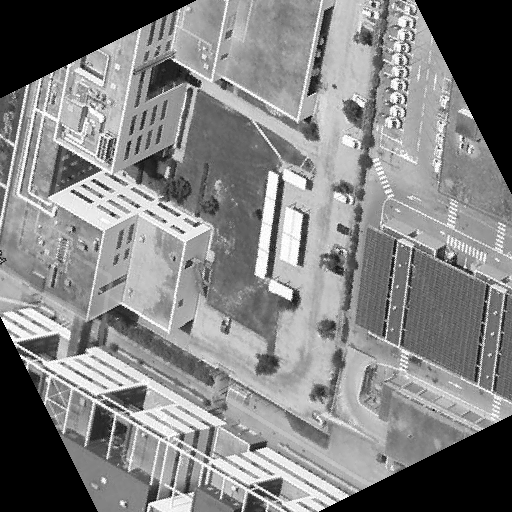
\includegraphics[scale=0.3]{../img/Q8_output_orig.png}
	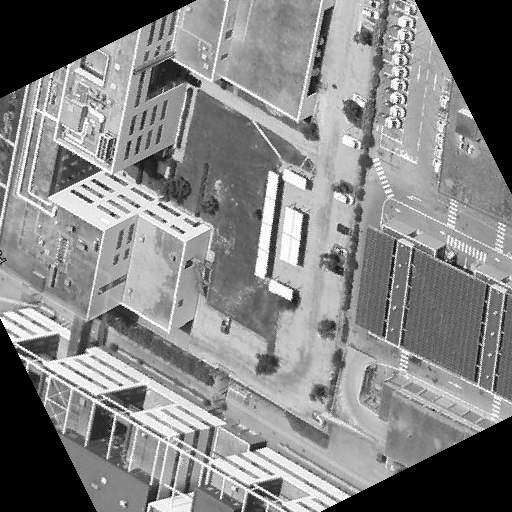
\includegraphics[scale=0.3]{../img/Q8_output.png}
\end{figure}
\begin{center}
L'image de gauche est générée par le programme rotation\_orig.\\
L'image de droite est générée par le programme rotation.
\end{center}


tx et ty représentent la taille d'une tuile selon l'axe x et l'axe y. \\


\section{Installation}
\subsection{ Installation du simulateur de cache}
\subsubsection{Question 9 :}

~
\begin{verbatim}
./dineroIV -informat d -l1-dbsize 64 -l1-dsize 16k -l1-dassoc 2
\end{verbatim}
dineroIV : Programme appelé.\\
informat : Sélectionne le format de la trace d'entrée. d : traditional din\\
l1-dbsize 6 : Fixe la taille d'une ligne de cache à 64 octets.\\
l1-dsize 16 : Fixe la taille du cache à 16 ko.\\
l1-dassoc : Fixe l'associativité du cache à 2.\\
	%_fin\end{lstlisting} : signifie que la suite de caractères ``_fin'' indique la fin de la
	%saisie.\\



	\subsubsection{Question 10 :}

	Sur l'image suivante, on voit le résultat de la commande dineroIV. On lit
	que quatre données ont été chargées (Total Demand Fetches : 4) ce qui
	correspond aux quatre lignes entrées avant \textit{\_fin}\\
	Le taux de miss est aussi cohérent : il est indiqué valoir 50\%. En effet,
	les deux miss (sur nos quatre accès) sont : le premier accès à l'adresse 0x0
	(compulsory miss) et l'accès à l'adresse 0x40 (compulsory miss aussi car
	juste après la taille d'une ligne de cache)
\begin{figure}[h]
	\centering
	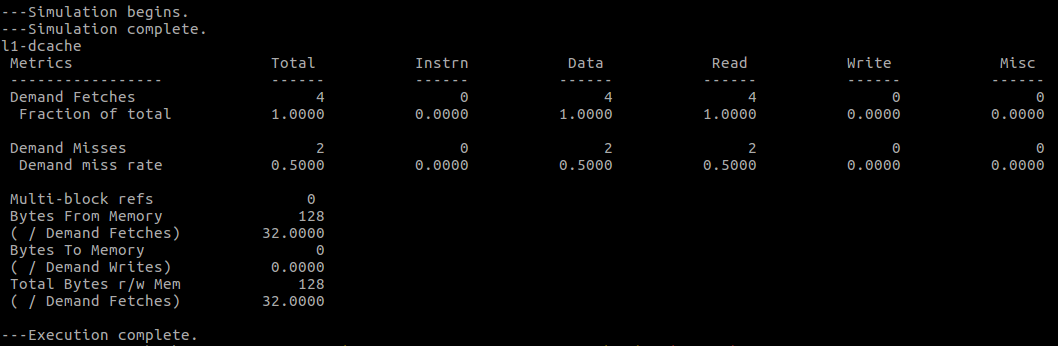
\includegraphics[scale=0.4]{../img/Q10_dineroIV_output.png}
	%\caption{The three founders. From left to right : the CTO, the
	%CEO, the COO}
	%\label{founders}
\end{figure}


	\subsubsection{Question 11 :}

	Le taux de réutilisation est obtenu en calculant le rapport entre la valeur
	obtenue par la commande suivante :
	\begin{verbatim}
		sort -u filename | wc -l
	\end{verbatim}
	 et celle obtenue par celle-ci :
	\begin{verbatim}
		wc -l filename
	\end{verbatim}

	\subsubsection{Question 12 :}

	Le taux de réutilisation de varie par lorsque la taille de la tuile varie
	car cela ne change le nombre d'opération effectuée.

	Avec tx=ty=1, pour un angle de 0 radian, on obtient un taux de 100\%
	(262144/262144) pour un angle de 0.52 randians, on obtient un taux de 88,36\%
	(191844/222154)
	
	Avec tx=ty=16, on obtient exactement les mêmes résultats que précédemment.

	\section{ Mesure de l’effet de la taille des tuiles}
	\subsection{Effet de l’angle de rotation sur les performances}
	\subsubsection{Question 13 :}

	Plus la tuile est grande, plus les données contenues dans une même ligne de
	cache sont accédées de manière successives. Ainsi, le taux de miss diminue
	quand la tuile augmente tant que la taille de la tuile demeure inférieure à
	la taille d'une ligne de cache (64 octets) : il est donc normal d'obtenir un
	pic de cache miss au-delà 64.

	\begin{figure}[h]
		\centering
		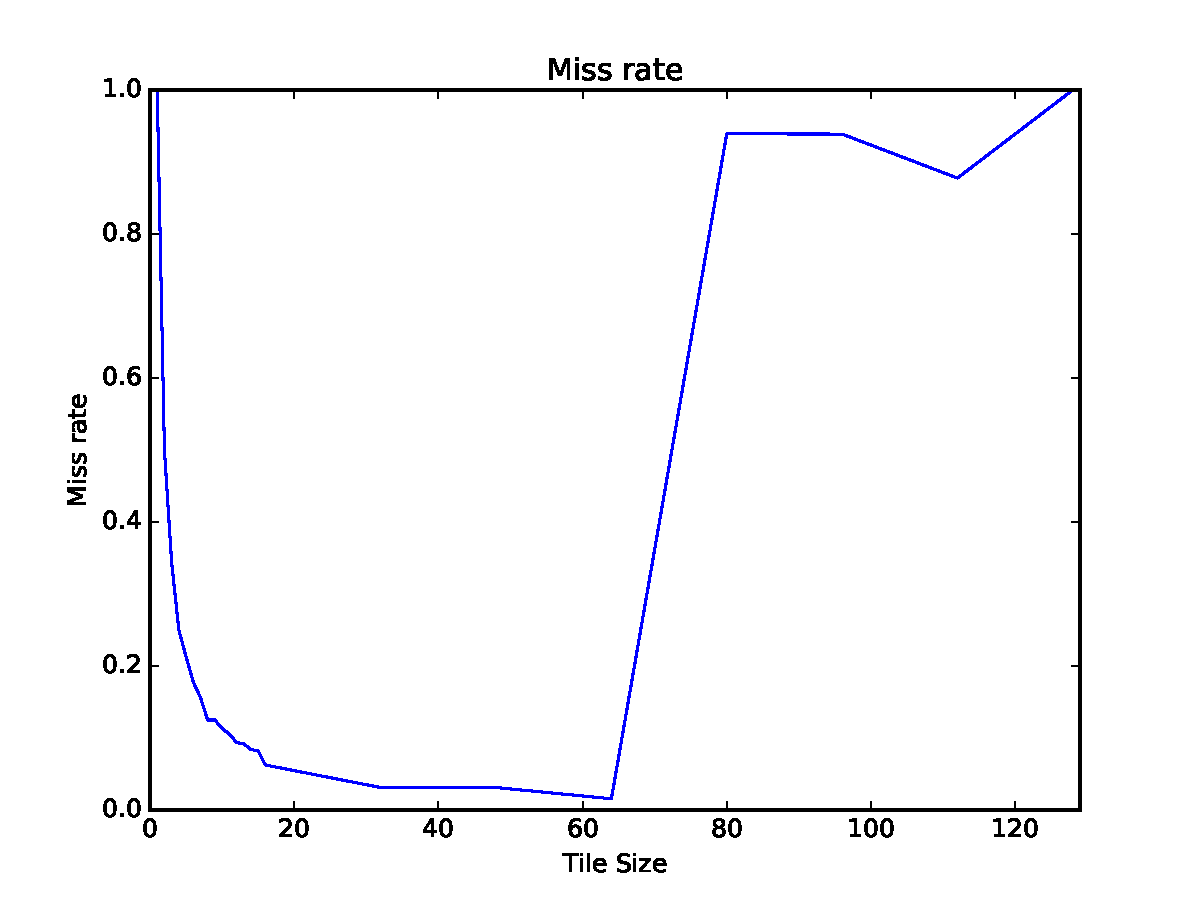
\includegraphics[width=0.9\linewidth]{../res/expe_simple}
		\caption{Alpha=0}
	\end{figure}


	\newpage
	\subsubsection{Question 14 :}

	Avec une rotation de 1,57 radians ($ \pi/ 2 $) lorsqu'on lit une colonne
	dont les valeurs se trouvent dans une ligne de cache, il y a écriture de ces
	même valeurs mais de manière horizontale d'où miss rate très faible.
	\begin{figure}[h]
		\centering
		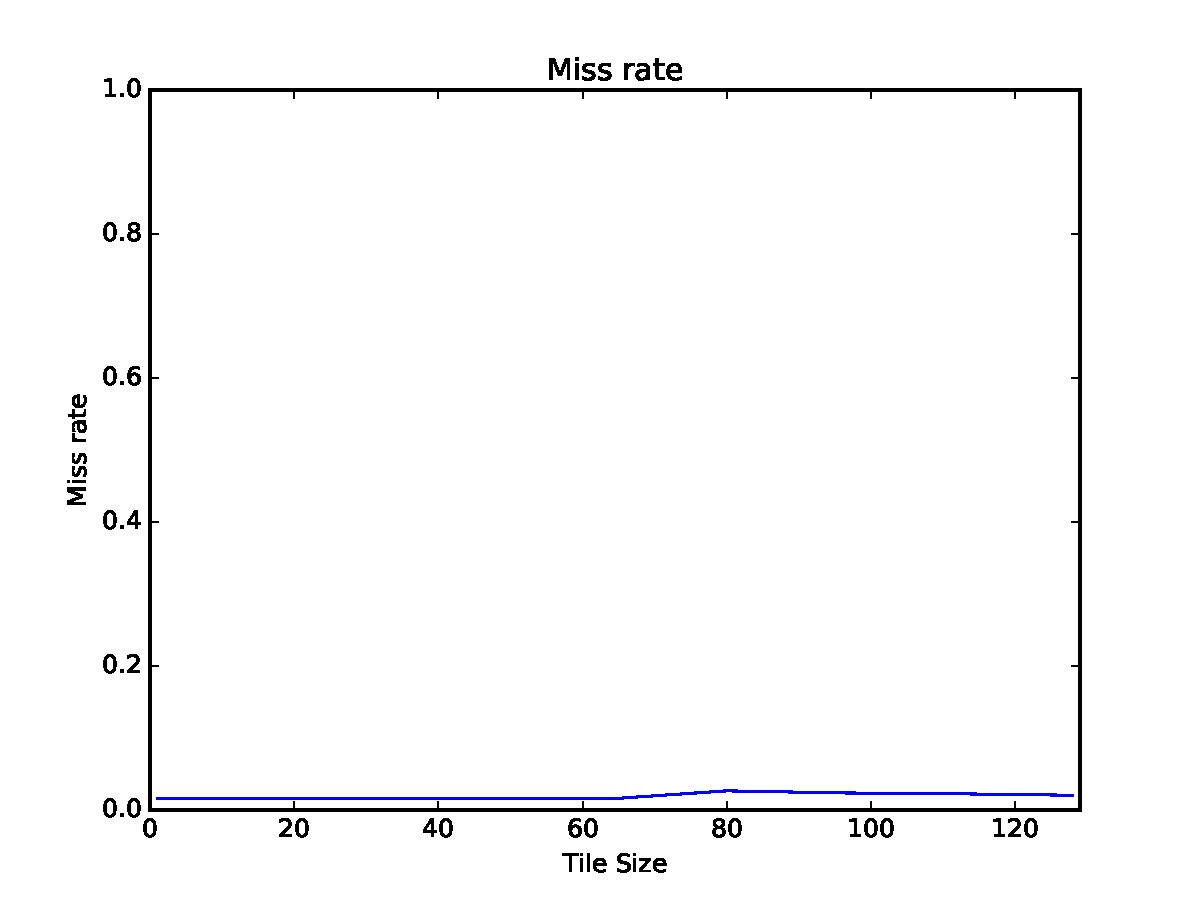
\includegraphics[width=0.9\linewidth]{../res/expe_simple1_57.pdf}
		\caption{Alpha=1.57}
	\end{figure}

	\subsection{Influence des paramètres du cache}
	\subsection{Question 15 :}

	\subsection{Impact du schéma d’adressage}
	\subsection{Question 16 :}

	\begin{figure}[h]
		\centering
		\begin{tabular}{|l|c|c|c|c|r|}
			\hline
			Coordonnées (x,y) & (0,0) & (1,0) & ... & (31,0) & (32,0) \\
			\hline
			Adresse de stockage & 0 & 1 & ... & 31 & 64 \\
			\hline
			Coordonnées (x,y) & (0,1) & (1,1) & ... & (31,1) & (32,1) \\
			\hline
			Adresse de stockage & 32 & 33 & ... & 63 & 96 \\
			\hline
		\end{tabular}
		\caption{Représentation des adresses de stockage}
	\end{figure}

	Une ligne de cache contient bien une fenêtre de taille 32x2.

	\subsection{Question 17 :}

	\subsection{Question 18 :}

	\section{Transformation de boucle}
	\subsection{Question 19 :}

	\subsection{Question 20 :}

	\section{Hiérarchie mémoire}
	\subsection{Question 21 :}

	\subsection{Question 22 :}
	%\begin{figure}[htbp]
		%\centering
		%%\includegraphics[width=0.9\linewidth]{../res/expe_simple_OBL}
		%\caption{Alpha=0}
		%\label{fig:1}
	%\end{figure}
	%\begin{figure}[htbp]
		%\centering
		%%\includegraphics[width=0.9\linewidth]{../res/expe_simple_1}
		%\caption{Alpha=0}
		%\label{fig:0}
	%\end{figure}
	%\begin{figure}[htbp]
		%\centering
		%\includegraphics[width=0.9\linewidth]{../res/expe_simple_1_OBL}
		%\caption{Alpha=0}
		%\label{fig:1}
	%\end{figure}
	\end{document}
